\documentclass[12pt]{standalone}
\usepackage[utf8]{inputenc}
\usepackage[T1]{fontenc}
\usepackage{times}
\usepackage{amsmath,amssymb}
\usepackage[dvipsnames,svgnames]{xcolor}
\usepackage{tikz}
\usetikzlibrary{decorations.pathreplacing, calc, positioning, shapes.geometric, shapes.symbols, arrows.meta, backgrounds, fit, shapes.misc}
\definecolor{RED}{rgb}{1,0,0}
\definecolor{dmrsfill}{HTML}{CDE2FB}
\definecolor{winblue}{HTML}{0D366B}
\definecolor{inksec}{HTML}{52514E}
\begin{document}
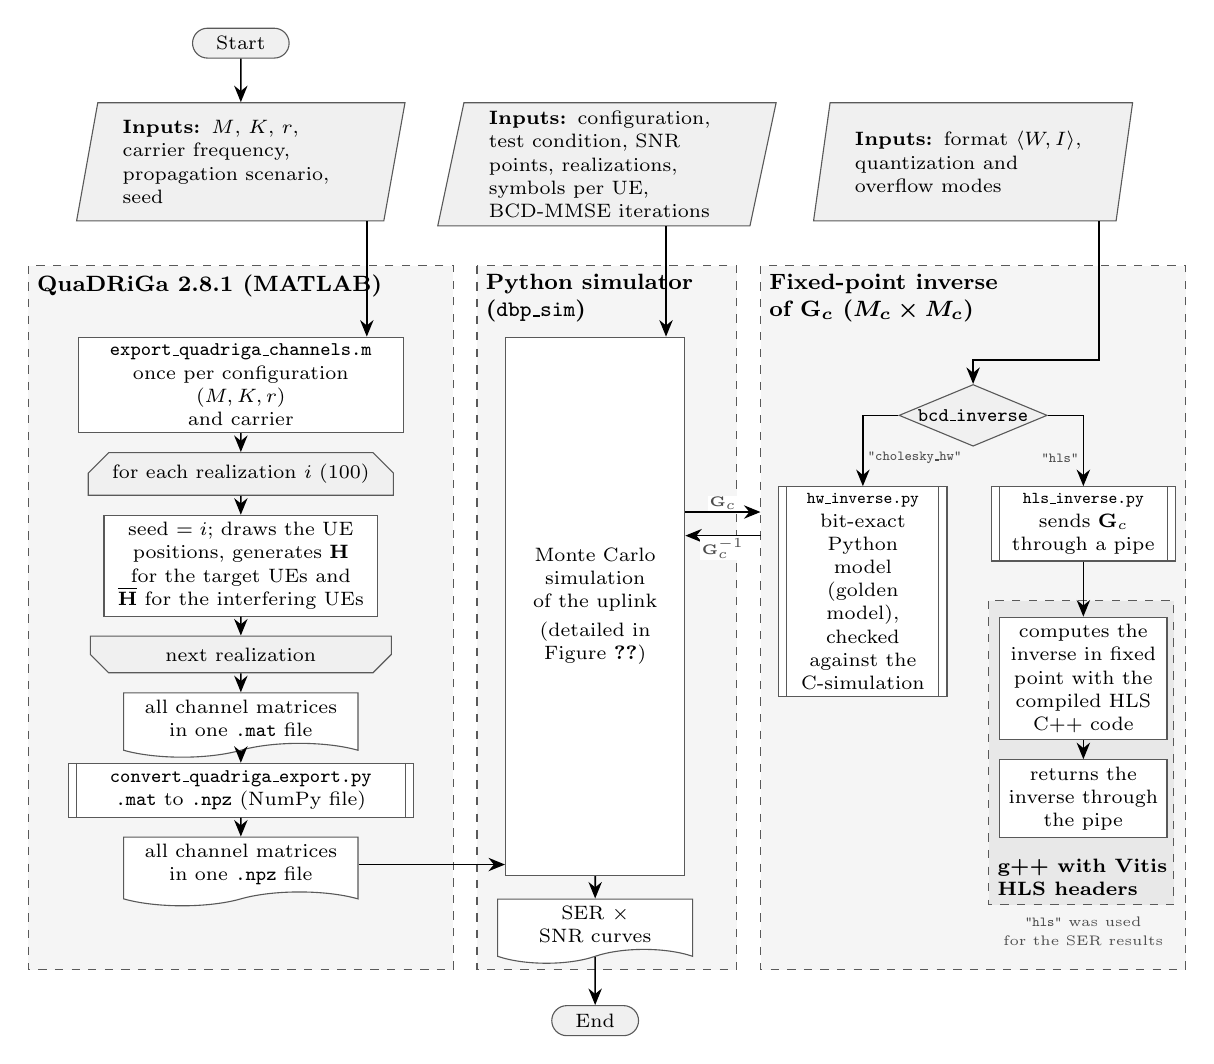
\begin{tikzpicture}[
  font=\fontsize{7}{8.4}\selectfont,
  >={Stealth[length=2.1mm, width=1.7mm]},
  node distance=2.4mm,
  box/.style={draw=black!65, fill=white, align=center,
              inner sep=2.5pt, text width=#1,
              execute at begin node={\hyphenpenalty=10000}},
  box/.default=4.9cm,
  inp/.style={trapezium, trapezium left angle=78, trapezium right angle=102,
              trapezium stretches body, draw=black!65, fill=black!6,
              align=left, inner xsep=9pt, inner ysep=3pt},
  arq/.style={tape, tape bend top=none, draw=black!65, fill=white, align=center,
              text width=#1, inner sep=2.5pt},
  pre/.style={box=#1, inner xsep=2.5pt+1.3mm,
              append after command={
                ($(\tikzlastnode.north west)+(1.1mm,0)$) edge[draw=black!65, -]
                ($(\tikzlastnode.south west)+(1.1mm,0)$)
                ($(\tikzlastnode.north east)+(-1.1mm,0)$) edge[draw=black!65, -]
                ($(\tikzlastnode.south east)+(-1.1mm,0)$)}},
  lini/.style={chamfered rectangle, chamfered rectangle corners={north west, north east},
              chamfered rectangle xsep=2mm, chamfered rectangle ysep=0.6mm,
              draw=black!65, fill=black!6, align=center, inner sep=2.5pt, text width=#1},
  lini/.default=4.2cm,
  lfim/.style={lini=#1, chamfered rectangle corners={south west, south east}},
  lfim/.default=4.2cm,
  term/.style={rounded rectangle, draw=black!65, fill=black!6, align=center,
              inner xsep=8pt, inner ysep=3pt},
  dec/.style={diamond, aspect=3.2, draw=black!65, fill=black!6, align=center, inner sep=0.5pt},
  ponto/.style={circle, draw=black!65, fill=white, minimum size=2.2mm, inner sep=0pt},
  cont/.style={draw=black!65, dashed, fill=black!4},
  tit/.style={anchor=north west, font=\fontsize{8}{9.6}\selectfont\bfseries\boldmath, align=left, inner sep=3pt},
  seta/.style={->, draw=black, line width=0.6pt},
  rot/.style={font=\fontsize{5.5}{6.6}\selectfont, text=black!70, inner sep=1.5pt},
]

% Colunas: QuaDRiGa [0; 5,4], Python [5,7; 9,0] (mais estreita, só um bloco),
%   inversa [9,3; 14,7]; 0,3 cm entre elas. Caixas tracejadas com a mesma altura;
%   entradas com o mesmo tamanho e alinhadas; setas das entradas à direita do centro
%   de cada coluna (fora dos títulos).
% =====================================================================
% Entradas
% =====================================================================
\begin{scope}[ent/.style={inp, anchor=north, text width=3.0cm, minimum height=1.5cm,
                           execute at begin node={\hyphenpenalty=10000\raggedright}}]
\node[term] (ini) at (2.7,0.75) {Start};
\node[ent] (inq) at (2.7,0) {\textbf{Inputs:} $M$, $K$, $r$, carrier frequency, propagation scenario, seed};
\node[ent] (ins) at (7.35,0) {\textbf{Inputs:} configuration, test condition, SNR points, realizations, symbols per UE, BCD-MMSE iterations};
\node[ent] (inf) at (12.0,0) {\textbf{Inputs:} format $\langle W, I\rangle$, quantization and overflow modes};
\end{scope}

% topo do conteúdo das colunas (as caixas tracejadas começam 9 mm acima)
\path let \p1=(ins.south) in coordinate (topo) at (7.35,\y1-14mm);

% =====================================================================
% QuaDRiGa (coluna da esquerda)
% =====================================================================
\path let \p1=(topo) in
  node[box=3.95cm, anchor=north] (exp) at (2.7,\y1) {\texttt{export\_quadriga\_channels.m}\\ once per configuration $(M, K, r)$\\ and carrier};
\node[lini=3.3cm, below=of exp] (lq) {for each realization $i$ (100)};
\node[box=3.3cm, below=of lq] (rea) {\mbox{seed $= i$}; draws the UE positions, generates $\mathbf{H}$ for the target UEs and $\overline{\mathbf{H}}$ for the interfering UEs};
\node[lfim=3.3cm, below=of rea] (lqf) {next realization};
\node[arq=2.8cm, below=of lqf] (mat) {all channel matrices\\ in one \texttt{.mat} file};
\node[pre=3.95cm, below=of mat] (cnv) {\texttt{convert\_quadriga\_export.py}\\ \texttt{.mat} to \texttt{.npz} (NumPy file)};
\node[arq=2.8cm, below=of cnv] (npz) {all channel matrices\\ in one \texttt{.npz} file};

\draw[seta] (ini) -- (inq);
\draw[seta] let \p1=(inq.south), \p2=(exp.north) in (4.3,\y1) -- (4.3,\y2);
\draw[seta] (exp) -- (lq);
\draw[seta] (lq) -- (rea);
\draw[seta] (rea) -- (lqf);
\draw[seta] (lqf) -- (mat);
\draw[seta] (mat) -- (cnv);
\draw[seta] (cnv) -- (npz);

% =====================================================================
% Inversa em ponto fixo (coluna da direita)
% =====================================================================
\path let \p1=(topo) in
  node[dec, aspect=2.4] (bcdi) at (12.0,\y1-1.0cm) {\texttt{bcd\_inverse}};
\path let \p1=(bcdi.south) in
  node[pre=1.9cm, anchor=north] (hls) at (13.4,\y1-5mm) {{\fontsize{6.2}{7.4}\selectfont\texttt{hls\_inverse.py}}\\ sends $\mathbf{G}_c$\\ through a pipe};
\path let \p1=(bcdi.south) in
  node[pre=1.7cm, anchor=north] (gold) at (10.6,\y1-5mm) {{\fontsize{6.2}{7.4}\selectfont\texttt{hw\_inverse.py}}\\ bit-exact Python model (golden model), checked against the C-simulation};
\node[box=1.95cm, below=7mm of hls] (cfx) {computes the inverse in fixed point with the compiled HLS C++ code};
\node[box=1.95cm, below=of cfx] (dev) {returns the inverse through the pipe};
\node[rot, align=center, below=9.5mm of dev] (uso) {\texttt{"hls"} was used\\ for the SER results};

\draw[seta] let \p1=(inf.south), \p2=(bcdi.north) in (13.6,\y1) -- (13.6,\y2+3mm) -- (\x2,\y2+3mm) -- (\p2);
\draw[seta] (bcdi.east) -| node[rot, pos=0.8, left] {\texttt{"hls"}} (hls.north);
\draw[seta] (bcdi.west) -| node[rot, pos=0.8, right] {\texttt{"cholesky\_hw"}} (gold.north);
\draw[seta] (hls) -- (cfx);
\draw[seta] (cfx) -- (dev);

% fundo comum das três caixas tracejadas
\path let \p1=(npz.south), \p2=(uso.south), \n1={min(\y1,\y2)-2.5mm} in coordinate (fundo) at (7.35,\n1);

% =====================================================================
% Simulador em Python: um bloco (detalhado na Figura fig:fluxo_python)
% =====================================================================
\path let \p1=(fundo) in
  node[arq=2.3cm, anchor=south] (crv) at (7.2,\y1+2.5mm) {SER $\times$ SNR curves};
\path let \p1=(topo), \p2=(crv.north), \n1={\y1-\y2-3mm} in
  node[box=2.1cm, anchor=north, minimum height=\n1] (py) at (7.2,\y1) {Monte Carlo\\ simulation\\ of the uplink\\[2pt] (detailed in\\ Figure~\ref{fig:fluxo_python})};
\node[term, below=7mm of crv] (fim) {End};

\draw[seta] let \p1=(ins.south), \p2=(py.north) in (8.1,\y1) -- (8.1,\y2);
\draw[seta] (py) -- (crv);
\draw[seta] (crv) -- (fim);

% canais do QuaDRiGa para o simulador
\draw[seta] (npz.east) -- (npz.east -| py.west);

% inversa: simulador (BCD-MMSE update) <-> coluna da direita
\draw[seta] let \p1=(py.east), \p2=(hls) in (\x1,\y2+1.5mm) -- node[rot, above, fill=white, inner sep=0.6pt, pos=0.5] {$\mathbf{G}_c$} (9.3,\y2+1.5mm);
\draw[seta] let \p1=(py.east), \p2=(hls) in (9.3,\y2-1.5mm) -- node[rot, below, fill=white, inner sep=0.6pt, pos=0.5] {$\mathbf{G}_c^{-1}$} (\x1,\y2-1.5mm);

% =====================================================================
% Caixas tracejadas (fundo)
% =====================================================================
\begin{scope}[on background layer]
  \path let \p1=(topo) in coordinate (qt) at (0,\y1+9mm);
  \draw[cont] (qt) rectangle (5.4,0 |- fundo);
  \node[tit] at (qt) {QuaDRiGa 2.8.1 (MATLAB)};

  \path let \p1=(topo) in coordinate (rt) at (5.7,\y1+9mm);
  \draw[cont] (rt) rectangle (9.0,0 |- fundo);
  \node[tit] at (rt) {Python simulator\\ (\texttt{dbp\_sim})};

  \path let \p1=(topo) in coordinate (it) at (9.3,\y1+9mm);
  \draw[cont] (it) rectangle (14.7,0 |- fundo);
  \node[tit] at (it) {Fixed-point inverse\\ of $\mathbf{G}_c$ ($M_c \times M_c$)};

  \path let \p1=(cfx.north), \p2=(dev.south) in
    coordinate (vt) at (12.2,\y1+2mm) coordinate (vb) at (14.55,\y2-8.5mm);
  \draw[cont, fill=black!9] (vt) rectangle (vb);
  \node[tit, font=\fontsize{7}{8.4}\selectfont\bfseries, anchor=south west] at (vt |- vb) {g++ with Vitis\\ HLS headers};
\end{scope}

\end{tikzpicture}
\end{document}
